\subsection{Suffix Array Konstruktion am Beispiel Banane}
\label{gsaca:chapter3}
%
Nachdem im vorherigen Kapitel das Vorgehen beschrieben wurde, wird in diesem Kapitel das Suffix Array für das kurze Beispielwort Banane konstruiert.
Dazu wird der Algorithmus schrittweise durchlaufen und die jeweiligen Zustände in tabellarischer Form visualisiert.

\subsection*{Phase 1:}
In der ersten Phase werden die Gruppen und Gruppenkontexte für das Wort Banane erstellt. 
Dies geschieht in insgesamt vier Iterationen.\\

Iteration 1:\\
Schritt 1: Das Wort Banane besteht aus vier verschiedenen Buchstaben (\textit{a}, \textit{b}, \textit{e}, \textit{n}), zusammen mit dem Terminalsymbol \textit{\$} sind somit am Beginn der ersten Iteration fünf Gruppen vorhanden. 
Die Tabelle \ref{fig_banane_1_1} zeigt den Ausgangszustand.
In ihr sind in der oberen Hälfte die initialen Gruppen und Gruppenkontexte dargestellt und in der unteren Hälfte das Wort zusammen mit den Indices der Buchstaben. 
Die initialen Gruppenkontexte sind die einzelnen Buchstaben.
Diese bestimmen auch die anfänglichen Gruppen, welche die Indices der Buchstaben im Wort beinhalten.
Der Algorithmus beginnt, indem der lexikographisch letzte Gruppenkontext betrachtet wird. 
In diesem Fall ist das der Buchstabe \textit{n}, welcher an den Indices 3 und 5 in dem Wort vorkommt. 
Die entsprechenden Zellen der Tabelle sind grün hervorgehoben. \\
Schritt 2: Dann werden die Vorkommen der aktuell betrachteten Gruppe im Wort untersucht. 
In dieser ersten Iteration ist es das Vorkommen von dem Zei\-chen \textit{n} an den Positionen 3 und 5. \\
Schritt 3: Danach werden die direkten Vorgänger im Wort untersucht. 
In diesem Schritt ist das der Buchstabe \textit{a} an den Positionen 2 und 4. 
Diese Indices sind zusammen mit den Buchstaben an den entsprechenden Positionen in der Tabelle rot hinterlegt. \\
Schritt 4: Im letzten Schritt dieser Iteration wird der Gruppenkontext der im vorherigen Schritt markierten Buchstaben betrachtet.
Dieser wird um den Kontext der Gruppe \textit{n} erweitert. 
Da alle Vorkommen der Gruppe \textit{a} Vorgänger von der Gruppe \textit{n} waren, findet diese Kontexterweiterung bei allen Elementen statt. 
Somit wird aus der Gruppe \textit{a} die Gruppe \textit{an}. Das finale Ergebnis zeigt die Änderungen vor gelben Hintergrund an.\\

Iteration 2:\\
Schritt 1: In der zweiten Iteration, deren Schritte in Tabelle \ref{gsaca:fig_banane_1_2} verdeutlicht werden, wird die nächste Gruppe bezüglich der lexikographisch absteigenden Ordnung betrachtet. 
Dies ist die Gruppe mit Kontext \textit{e}.\\
Schritt 2: Der Buchstabe \textit{e} kommt nur an Index 6 im Wort vor.\\
Schritt 3: Für diesen Index wird die Vorgängergruppe gesucht. 
Diese ist die Gruppe \textit{an}, die im vorherigen Schritt gebildet wurde.\\
Schritt 4: Anders als in der vorherigen Iteration werden in diesem Durchlauf nicht alle Vorkommen der Vorgängergruppe getroffen. 
Damit muss diese Gruppe in zwei neue Gruppen aufgeteilt werden. 
Der erste Teil der Gruppe bleibt \textit{an} und der zweite Teil wird um den Kontext von \textit{e} erweitert. 
Da die Gruppe mit dem erweiterten Kontext lexikographisch größer ist, wird sie zum neuen Nachfolger der Teilgruppe ohne Kontexterweiterung.\\

Iteration 3:\\
Schritt 1: Als nächstes wird die Gruppe \textit{b} betrachtet. 
Die Zwischenergebnisse dieser Iteration sind in Tabelle \ref{fig_banane_1_3} zu sehen.\\
Schritt 2: Diese Gruppe hat keinen Vorgänger im betrachteten Wort. 
Daher endet diese Iteration ohne Änderungen an den Kontextgruppen.\\

Iteration 4: \\
Schritt 1: Es wird die nächste Gruppe betrachtet. Dies ist die Gruppe mit Kontext \textit{ane}.\\
Schritt 2: Diese Gruppe umfasst die Indices 4 bis 6 im Wort Banane.\\
Schritt 3: Der Vorgänger dieser Gruppe ist die Gruppe \textit{an}.\\
Schritt 4: Wie in der ersten Iteration wird die gesamte Vorgängergruppe getroffen. 
Diese wird um den Kontext der Gruppe \textit{ane} erweitert. 
Das Ergebnis dieser Iteration und der gesamten Phase 1 ist in Tabelle \ref{fig_banane_1_4} gezeigt. 
Am Ende dieser Phase hat man somit 6 Gruppenkontexte: \textit{\$}, \textit{anane}, \textit{ane}, \textit{b}, \textit{e} und \textit{n}. 
Zusätzlich wurden für alle Buchstaben des Wortes die \prevpointer erzeugt und gespeichert. 
Die entstandenen Pointer-Ketten lassen sich in Abbildung \ref{fig_banane_prev_pointer} sehen. 
Auf diesem Ergebnis aufbauend wird in Phase 2 das finale Suffix-Array berechnet werden.
\newpage		% start new page to align tables on top of next page

%%%%%%%%%%% Phase 1 %%%%%%%%%%%%%%%
\begin{table}[H]

\centering
\begin{adjustbox}{max width=\textwidth}
\begin{tabular}{ll}

% Phase 1 - Iteration 1 - Schritt 1
\begin{tabular}{lccccccc}
\multicolumn{8}{l}{Phase 1 - Iteration 1 - Schritt 1}                                                                                                                                         \\ \hline
\multicolumn{1}{l|}{Kontext} & \multicolumn{1}{c|}{\$} & \multicolumn{2}{c|}{a}     & \multicolumn{1}{c|}{b} & \multicolumn{1}{c|}{e} & \multicolumn{2}{c}{\cellcolor[HTML]{\green}n}        \\
\multicolumn{1}{l|}{Gruppe}  & \multicolumn{1}{c|}{7}  & 2 & \multicolumn{1}{c|}{4} & \multicolumn{1}{c|}{1} & \multicolumn{1}{c|}{6} & \cellcolor[HTML]{\green}3 & \cellcolor[HTML]{\green}5 \\ \hline
\multicolumn{1}{l|}{Index}   & 1                       & 2 & 3                      & 4                      & 5                      & 6                         & 7                         \\
\multicolumn{1}{l|}{Zeichen} & b                       & a & n                      & a                      & n                      & e                         & \$                       
\end{tabular}

&

% Phase 1 - Iteration 1 - Schritt 2
\begin{tabular}{lccccccc}
\multicolumn{8}{l}{Phase 1 - Iteration 1 - Schritt 2}                                                                                                                                               \\ \hline
\multicolumn{1}{l|}{Kontext} & \multicolumn{1}{c|}{\$} & \multicolumn{2}{c|}{a}        & \multicolumn{1}{c|}{b} & \multicolumn{1}{c|}{e}    & \multicolumn{2}{c}{\cellcolor[HTML]{\green}n}         \\
\multicolumn{1}{l|}{Gruppe}  & \multicolumn{1}{c|}{7}  & 2 & \multicolumn{1}{c|}{4}    & \multicolumn{1}{c|}{1} & \multicolumn{1}{c|}{6}    & \cellcolor[HTML]{\green}3 & \cellcolor[HTML]{\green}5 \\ \hline
\multicolumn{1}{l|}{Index}   & 1                       & 2 & \cellcolor[HTML]{\green}3 & 4                      & \cellcolor[HTML]{\green}5 & 6                         & 7                         \\
\multicolumn{1}{l|}{Zeichen} & b                       & a & \cellcolor[HTML]{\green}n & a                      & \cellcolor[HTML]{\green}n & e                         & \$                       
\end{tabular}

\\
&
\\

% Phase 1 - Iteration 1 - Schritt 3
\begin{tabular}{lccccccc}
\multicolumn{8}{l}{Phase 1 - Iteration 1 - Schritt 3}                                                                                                                                                                          \\ \hline
\multicolumn{1}{l|}{Kontext} & \multicolumn{1}{c|}{\$} & \multicolumn{2}{c|}{a}                                & \multicolumn{1}{c|}{b}    & \multicolumn{1}{c|}{e}    & \multicolumn{2}{c}{\cellcolor[HTML]{\green}n}         \\
\multicolumn{1}{l|}{Gruppe}  & \multicolumn{1}{c|}{7}  & 2                         & \multicolumn{1}{c|}{4}    & \multicolumn{1}{c|}{1}    & \multicolumn{1}{c|}{6}    & \cellcolor[HTML]{\green}3 & \cellcolor[HTML]{\green}5 \\ \hline
\multicolumn{1}{l|}{Index}   & 1                       & \cellcolor[HTML]{\red}2 & \cellcolor[HTML]{\green}3 & \cellcolor[HTML]{\red}4 & \cellcolor[HTML]{\green}5 & 6                         & 7                         \\
\multicolumn{1}{l|}{Zeichen} & b                       & \cellcolor[HTML]{\red}a & \cellcolor[HTML]{\green}n & \cellcolor[HTML]{\red}a & \cellcolor[HTML]{\green}n & e                         & \$                       
\end{tabular}

&

% Phase 1 - Iteration 1 - Schritt 4
\begin{tabular}{lccccccc}
\multicolumn{8}{l}{Phase 1 - Iteration 1 - Schritt 4}                                                                                                                                                                                               \\ \hline
\multicolumn{1}{l|}{Kontext} & \multicolumn{1}{c|}{\$} & \multicolumn{2}{c|}{\cellcolor[HTML]{\red}a}                             & \multicolumn{1}{c|}{b}    & \multicolumn{1}{c|}{e}    & \multicolumn{2}{c}{\cellcolor[HTML]{\green}n}         \\
\multicolumn{1}{l|}{Gruppe}  & \multicolumn{1}{c|}{7}  & \cellcolor[HTML]{\red}2 & \multicolumn{1}{c|}{\cellcolor[HTML]{\red}4} & \multicolumn{1}{c|}{1}    & \multicolumn{1}{c|}{6}    & \cellcolor[HTML]{\green}3 & \cellcolor[HTML]{\green}5 \\ \hline
\multicolumn{1}{l|}{Index}   & 1                       & \cellcolor[HTML]{\red}2 & \cellcolor[HTML]{\green}3                      & \cellcolor[HTML]{\red}4 & \cellcolor[HTML]{\green}5 & 6                         & 7                         \\
\multicolumn{1}{l|}{Zeichen} & b                       & \cellcolor[HTML]{\red}a & \cellcolor[HTML]{\green}n                      & \cellcolor[HTML]{\red}a & \cellcolor[HTML]{\green}n & e                         & \$                       
\end{tabular}

\\
&
\\

% Phase 1 - Iteration 1 - Ergebnis
\begin{tabular}{lccccccc}
\multicolumn{8}{l}{Phase 1 - Iteration 1 - Ergebnis}                                                                                                                                                          \\ \hline
\multicolumn{1}{l|}{Kontext} & \multicolumn{1}{c|}{\$} & \multicolumn{2}{c|}{\cellcolor[HTML]{\yellow}an}                            & \multicolumn{1}{c|}{b} & \multicolumn{1}{c|}{e} & \multicolumn{2}{c}{n} \\
\multicolumn{1}{l|}{Gruppe}  & \multicolumn{1}{c|}{7}  & \cellcolor[HTML]{\yellow}2 & \multicolumn{1}{c|}{\cellcolor[HTML]{\yellow}4} & \multicolumn{1}{c|}{1} & \multicolumn{1}{c|}{6} & 3         & 5         \\ \hline
\multicolumn{1}{l|}{Index}   & 1                       & 2                         & 3                                              & 4                      & 5                      & 6         & 7         \\
\multicolumn{1}{l|}{Zeichen} & b                       & a                         & n                                              & a                      & n                      & e         & \$       
\end{tabular}

\end{tabular}
\end{adjustbox}

\caption[Konstruktion des Suffix-Arrays für das Wort Banane: Phase 1, Iteration 1]{Konstruktion des Suffix-Arrays für das Wort Banane: Phase 1, Iteration 1}
\label{fig_banane_1_1} 
\end{table}

\begin{table}[H]

\centering
\begin{adjustbox}{max width=\textwidth}
\begin{tabular}{ll}

% Phase 1 - Iteration 2 - Schritt 1
\begin{tabular}{lccccccc}
\multicolumn{8}{l}{Phase 1 - Iteration 2 - Schritt 2}                                                                                                                                  \\ \hline
\multicolumn{1}{l|}{Kontext} & \multicolumn{1}{c|}{\$} & \multicolumn{2}{c|}{an}    & \multicolumn{1}{c|}{b} & \multicolumn{1}{c|}{\cellcolor[HTML]{\green}e} & \multicolumn{2}{c}{n} \\
\multicolumn{1}{l|}{Gruppe}  & \multicolumn{1}{c|}{7}  & 2 & \multicolumn{1}{c|}{4} & \multicolumn{1}{c|}{1} & \multicolumn{1}{c|}{\cellcolor[HTML]{\green}6} & 3         & 5          \\ \hline
\multicolumn{1}{l|}{Index}   & 1                       & 2 & 3                      & 4                      & 5                                              & 6         & 7          \\
\multicolumn{1}{l|}{Zeichen} & b                       & a & n                      & a                      & n                                              & e         & \$        
\end{tabular}

&

% Phase 1 - Iteration 2 - Schritt 2
\begin{tabular}{lccccccc}
\multicolumn{8}{l}{Phase 1 - Iteration 2 - Schritt 2}                                                                                                                                          \\ \hline
\multicolumn{1}{l|}{Kontext} & \multicolumn{1}{c|}{\$} & \multicolumn{2}{c|}{an}    & \multicolumn{1}{c|}{b} & \multicolumn{1}{c|}{\cellcolor[HTML]{\green}e} & \multicolumn{2}{c}{n}         \\
\multicolumn{1}{l|}{Gruppe}  & \multicolumn{1}{c|}{7}  & 2 & \multicolumn{1}{c|}{4} & \multicolumn{1}{c|}{1} & \multicolumn{1}{c|}{\cellcolor[HTML]{\green}6} & 3                         & 5  \\ \hline
\multicolumn{1}{l|}{Index}   & 1                       & 2 & 3                      & 4                      & 5                                              & \cellcolor[HTML]{\green}6 & 7  \\
\multicolumn{1}{l|}{Zeichen} & b                       & a & n                      & a                      & n                                              & \cellcolor[HTML]{\green}e & \$
\end{tabular}

\\
&
\\

% Phase 1 - Iteration 2 - Schritt 3
\begin{tabular}{lccccccc}
\multicolumn{8}{l}{Phase 1 - Iteration 2 - Schritt 3}                                                                                                                                             \\ \hline
\multicolumn{1}{l|}{Kontext} & \multicolumn{1}{c|}{\$} & \multicolumn{2}{c|}{an}    & \multicolumn{1}{c|}{b}    & \multicolumn{1}{c|}{\cellcolor[HTML]{\green}e} & \multicolumn{2}{c}{n}         \\
\multicolumn{1}{l|}{Gruppe}  & \multicolumn{1}{c|}{7}  & 2 & \multicolumn{1}{c|}{4} & \multicolumn{1}{c|}{1}    & \multicolumn{1}{c|}{\cellcolor[HTML]{\green}6} & 3                         & 5  \\ \hline
\multicolumn{1}{l|}{Index}   & 1                       & 2 & 3                      & \cellcolor[HTML]{\red}4 & \cellcolor[HTML]{\red}5                      & \cellcolor[HTML]{\green}6 & 7  \\
\multicolumn{1}{l|}{Zeichen} & b                       & a & n                      & \cellcolor[HTML]{\red}a & \cellcolor[HTML]{\red}n                      & \cellcolor[HTML]{\green}e & \$
\end{tabular}

&

% Phase 1 - Iteration 2 - Schritt 4
\begin{tabular}{lccccccc}
\multicolumn{8}{l}{Phase 1 - Iteration 2 - Schritt 4}                                                                                                                                                                     \\ \hline
\multicolumn{1}{l|}{Kontext} & \multicolumn{1}{c|}{\$} & \multicolumn{2}{c|}{\cellcolor[HTML]{\red}an}    & \multicolumn{1}{c|}{b}    & \multicolumn{1}{c|}{\cellcolor[HTML]{\green}e} & \multicolumn{2}{c}{n}         \\
\multicolumn{1}{l|}{Gruppe}  & \multicolumn{1}{c|}{7}  & 2 & \multicolumn{1}{c|}{\cellcolor[HTML]{\red}4} & \multicolumn{1}{c|}{1}    & \multicolumn{1}{c|}{\cellcolor[HTML]{\green}6} & 3                         & 5  \\ \hline
\multicolumn{1}{l|}{Index}   & 1                       & 2 & 3                                              & \cellcolor[HTML]{\red}4 & \cellcolor[HTML]{\red}5                      & \cellcolor[HTML]{\green}6 & 7  \\
\multicolumn{1}{l|}{Zeichen} & b                       & a & n                                              & \cellcolor[HTML]{\red}a & \cellcolor[HTML]{\red}n                      & \cellcolor[HTML]{\green}e & \$
\end{tabular}

\\
&
\\

% Phase 1 - Iteration 2 - Ergebnis
\begin{tabular}{lccccccc}
\multicolumn{8}{l}{Phase 1 - Iteration 2 - Schritt 4}                                                                                                                                                                                  \\ \hline
\multicolumn{1}{l|}{Kontext} & \multicolumn{1}{c|}{\$} & \multicolumn{1}{c|}{\cellcolor[HTML]{\yellow}an} & \multicolumn{1}{c|}{\cellcolor[HTML]{\yellow}ane} & \multicolumn{1}{c|}{b} & \multicolumn{1}{c|}{e} & \multicolumn{2}{c}{n} \\
\multicolumn{1}{l|}{Gruppe}  & \multicolumn{1}{c|}{7}  & \multicolumn{1}{c|}{\cellcolor[HTML]{\yellow}2}  & \multicolumn{1}{c|}{\cellcolor[HTML]{\yellow}4}   & \multicolumn{1}{c|}{1} & \multicolumn{1}{c|}{6} & 3         & 5          \\ \hline
\multicolumn{1}{l|}{Index}   & 1                       & 2                                               & 3                                                & 4                      & 5                      & 6         & 7          \\
\multicolumn{1}{l|}{Zeichen} & b                       & a                                               & n                                                & a                      & n                      & e         & \$        
\end{tabular}

\end{tabular}
\end{adjustbox}

\caption[Konstruktion des Suffix Arrays für das Wort Banane: Phase 1, Iteration 2]{Konstruktion des Suffix Arrays für das Wort Banane: Phase 1, Iteration 2}
\label{gsaca:fig_banane_1_2} 
\end{table}

\newpage 		% start new page to remove space between tables
\begin{table}[H]

\centering
\begin{adjustbox}{max width=\textwidth}
\begin{tabular}{ll}

% Phase 1 - Iteration 3 - Schritt 1
\begin{tabular}{lccccccc}
\multicolumn{8}{l}{Phase 1 - Iteration 3 - Schritt 1}                                                                                                                                                          \\ \hline
\multicolumn{1}{l|}{Kontext} & \multicolumn{1}{c|}{\$} & \multicolumn{1}{c|}{an} & \multicolumn{1}{c|}{ane} & \multicolumn{1}{c|}{\cellcolor[HTML]{\green}b} & \multicolumn{1}{c|}{e} & \multicolumn{2}{c}{n} \\
\multicolumn{1}{l|}{Gruppe}  & \multicolumn{1}{c|}{7}  & \multicolumn{1}{c|}{2}  & \multicolumn{1}{c|}{4}   & \multicolumn{1}{c|}{\cellcolor[HTML]{\green}1} & \multicolumn{1}{c|}{6} & 3         & 5          \\ \hline
\multicolumn{1}{l|}{Index}   & 1                       & 2                       & 3                        & 4                                              & 5                      & 6         & 7          \\
\multicolumn{1}{l|}{Zeichen} & b                       & a                       & n                        & a                                              & n                      & e         & \$        
\end{tabular}

&

% Phase 1 - Iteration 3 - Schritt 2
\begin{tabular}{lccccccc}
\multicolumn{8}{l}{Phase 1 - Iteration 3 - Schritt 1}                                                                                                                                                            \\ \hline
\multicolumn{1}{l|}{Kontext} & \multicolumn{1}{c|}{\$}   & \multicolumn{1}{c|}{an} & \multicolumn{1}{c|}{ane} & \multicolumn{1}{c|}{\cellcolor[HTML]{\green}b} & \multicolumn{1}{c|}{e} & \multicolumn{2}{c}{n} \\
\multicolumn{1}{l|}{Gruppe}  & \multicolumn{1}{c|}{7}    & \multicolumn{1}{c|}{2}  & \multicolumn{1}{c|}{4}   & \multicolumn{1}{c|}{\cellcolor[HTML]{\green}1} & \multicolumn{1}{c|}{6} & 3         & 5          \\ \hline
\multicolumn{1}{l|}{Index}   & \cellcolor[HTML]{\green}1 & 2                       & 3                        & 4                                              & 5                      & 6         & 7          \\
\multicolumn{1}{l|}{Zeichen} & \cellcolor[HTML]{\green}b & a                       & n                        & a                                              & n                      & e         & \$        
\end{tabular}

\\
&
\\

% Phase 1 - Iteration 3 - Ergebnis
\begin{tabular}{lccccccc}
\multicolumn{8}{l}{Phase 1 - Iteration 3 - Schritt 1}                                                                                                                                  \\ \hline
\multicolumn{1}{l|}{Kontext} & \multicolumn{1}{c|}{\$} & \multicolumn{1}{c|}{an} & \multicolumn{1}{c|}{ane} & \multicolumn{1}{c|}{b} & \multicolumn{1}{c|}{e} & \multicolumn{2}{c}{n} \\
\multicolumn{1}{l|}{Gruppe}  & \multicolumn{1}{c|}{7}  & \multicolumn{1}{c|}{2}  & \multicolumn{1}{c|}{4}   & \multicolumn{1}{c|}{1} & \multicolumn{1}{c|}{6} & 3         & 5          \\ \hline
\multicolumn{1}{l|}{Index}   & 1                       & 2                       & 3                        & 4                      & 5                      & 6         & 7          \\
\multicolumn{1}{l|}{Zeichen} & b                       & a                       & n                        & a                      & n                      & e         & \$        
\end{tabular}

\end{tabular}
\end{adjustbox}

\caption[Konstruktion des Suffix Arrays f{\"u}r das Wort Banane: Phase 1, Iteration 3]{Konstruktion des Suffix Arrays f{\"u}r das Wort Banane: Phase 1, Iteration 3}
\label{fig_banane_1_3} 
\end{table}

\begin{table}[H]

\centering
\begin{adjustbox}{max width=\textwidth}
\begin{tabular}{ll}

% Phase 1 - Iteration 4 - Schritt 1
\begin{tabular}{lccccccc}
\multicolumn{8}{l}{Phase 1 - Iteration 4 - Schritt 1}                                                                                                                                                          \\ \hline
\multicolumn{1}{l|}{Kontext} & \multicolumn{1}{c|}{\$} & \multicolumn{1}{c|}{an} & \multicolumn{1}{c|}{\cellcolor[HTML]{\green}ane} & \multicolumn{1}{c|}{b} & \multicolumn{1}{c|}{e} & \multicolumn{2}{c}{n} \\
\multicolumn{1}{l|}{Gruppe}  & \multicolumn{1}{c|}{7}  & \multicolumn{1}{c|}{2}  & \multicolumn{1}{c|}{\cellcolor[HTML]{\green}4}   & \multicolumn{1}{c|}{1} & \multicolumn{1}{c|}{6} & 3         & 5          \\ \hline
\multicolumn{1}{l|}{Index}   & 1                       & 2                       & 3                                                & 4                      & 5                      & 6         & 7          \\
\multicolumn{1}{l|}{Zeichen} & b                       & a                       & n                                                & a                      & n                      & e         & \$        
\end{tabular}

&

% Phase 1 - Iteration 4 - Schritt 2
\begin{tabular}{lccccccc}
\multicolumn{8}{l}{Phase 1 - Iteration 4 - Schritt 2}                                                                                                                                                                        \\ \hline
\multicolumn{1}{l|}{Kontext} & \multicolumn{1}{c|}{\$} & \multicolumn{1}{c|}{an} & \multicolumn{1}{c|}{\cellcolor[HTML]{\green}ane} & \multicolumn{1}{c|}{b}    & \multicolumn{1}{c|}{e}    & \multicolumn{2}{c}{n}         \\
\multicolumn{1}{l|}{Gruppe}  & \multicolumn{1}{c|}{7}  & \multicolumn{1}{c|}{2}  & \multicolumn{1}{c|}{\cellcolor[HTML]{\green}4}   & \multicolumn{1}{c|}{1}    & \multicolumn{1}{c|}{6}    & 3                         & 5  \\ \hline
\multicolumn{1}{l|}{Index}   & 1                       & 2                       & 3                                                & \cellcolor[HTML]{\green}4 & \cellcolor[HTML]{\green}5 & \cellcolor[HTML]{\green}6 & 7  \\
\multicolumn{1}{l|}{Zeichen} & b                       & a                       & n                                                & \cellcolor[HTML]{\green}a & \cellcolor[HTML]{\green}n & \cellcolor[HTML]{\green}e & \$
\end{tabular}

\\
&
\\

% Phase 1 - Iteration 4 - Schritt 3
\begin{tabular}{lccccccc}
\multicolumn{8}{l}{Phase 1 - Iteration 4 - Schritt 3}                                                                                                                                                                          \\ \hline
\multicolumn{1}{l|}{Kontext} & \multicolumn{1}{c|}{\$} & \multicolumn{1}{c|}{an}   & \multicolumn{1}{c|}{\cellcolor[HTML]{\green}ane} & \multicolumn{1}{c|}{b}    & \multicolumn{1}{c|}{e}    & \multicolumn{2}{c}{n}         \\
\multicolumn{1}{l|}{Gruppe}  & \multicolumn{1}{c|}{7}  & \multicolumn{1}{c|}{2}    & \multicolumn{1}{c|}{\cellcolor[HTML]{\green}4}   & \multicolumn{1}{c|}{1}    & \multicolumn{1}{c|}{6}    & 3                         & 5  \\ \hline
\multicolumn{1}{l|}{Index}   & 1                       & \cellcolor[HTML]{\red}2 & \cellcolor[HTML]{\red}3                        & \cellcolor[HTML]{\green}4 & \cellcolor[HTML]{\green}5 & \cellcolor[HTML]{\green}6 & 7  \\
\multicolumn{1}{l|}{Zeichen} & b                       & \cellcolor[HTML]{\red}a & \cellcolor[HTML]{\red}n                        & \cellcolor[HTML]{\green}a & \cellcolor[HTML]{\green}n & \cellcolor[HTML]{\green}e & \$
\end{tabular}

&

% Phase 1 - Iteration 4 - Schritt 4
\begin{tabular}{lccccccc}
\multicolumn{8}{l}{Phase 1 - Iteration 4 - Schritt 4}                                                                                                                                                                                                \\ \hline
\multicolumn{1}{l|}{Kontext} & \multicolumn{1}{c|}{\$} & \multicolumn{1}{c|}{\cellcolor[HTML]{\red}an} & \multicolumn{1}{c|}{\cellcolor[HTML]{\green}ane} & \multicolumn{1}{c|}{b}    & \multicolumn{1}{c|}{e}    & \multicolumn{2}{c}{n}         \\
\multicolumn{1}{l|}{Gruppe}  & \multicolumn{1}{c|}{7}  & \multicolumn{1}{c|}{\cellcolor[HTML]{\red}2}  & \multicolumn{1}{c|}{\cellcolor[HTML]{\green}4}   & \multicolumn{1}{c|}{1}    & \multicolumn{1}{c|}{6}    & 3                         & 5  \\ \hline
\multicolumn{1}{l|}{Index}   & 1                       & \cellcolor[HTML]{\red}2                       & \cellcolor[HTML]{\red}3                        & \cellcolor[HTML]{\green}4 & \cellcolor[HTML]{\green}5 & \cellcolor[HTML]{\green}6 & 7  \\
\multicolumn{1}{l|}{Zeichen} & b                       & \cellcolor[HTML]{\red}a                       & \cellcolor[HTML]{\red}n                        & \cellcolor[HTML]{\green}a & \cellcolor[HTML]{\green}n & \cellcolor[HTML]{\green}e & \$
\end{tabular}

\\
&
\\

% Phase 1 - Iteration 4 - Ergebnis
\begin{tabular}{lccccccc}
\multicolumn{8}{l}{Phase 1 - Iteration 4 - Ergebnis}                                                                                                                                                              \\ \hline
\multicolumn{1}{l|}{Kontext} & \multicolumn{1}{c|}{\$} & \multicolumn{1}{c|}{\cellcolor[HTML]{\yellow}anane} & \multicolumn{1}{c|}{ane} & \multicolumn{1}{c|}{b} & \multicolumn{1}{c|}{e} & \multicolumn{2}{c}{n} \\
\multicolumn{1}{l|}{Gruppe}  & \multicolumn{1}{c|}{7}  & \multicolumn{1}{c|}{\cellcolor[HTML]{\yellow}2}     & \multicolumn{1}{c|}{4}   & \multicolumn{1}{c|}{1} & \multicolumn{1}{c|}{6} & 3         & 5          \\ \hline
\multicolumn{1}{l|}{Index}   & 1                       & 2                                                  & 3                        & 4                      & 5                      & 6         & 7          \\
\multicolumn{1}{l|}{Zeichen} & b                       & a                                                  & n                        & a                      & n                      & e         & \$        
\end{tabular}

\end{tabular}
\end{adjustbox}

\caption[Konstruktion des Suffix-Arrays für das Wort Banane: Phase 1, Iteration 4]{Konstruktion des Suffix-Arrays für das Wort Banane: Phase 1, Iteration 4}
\label{fig_banane_1_4} 
\end{table}


\begin{figure}[!b]
	\begin{minipage}[H]{10cm}
		\centering
		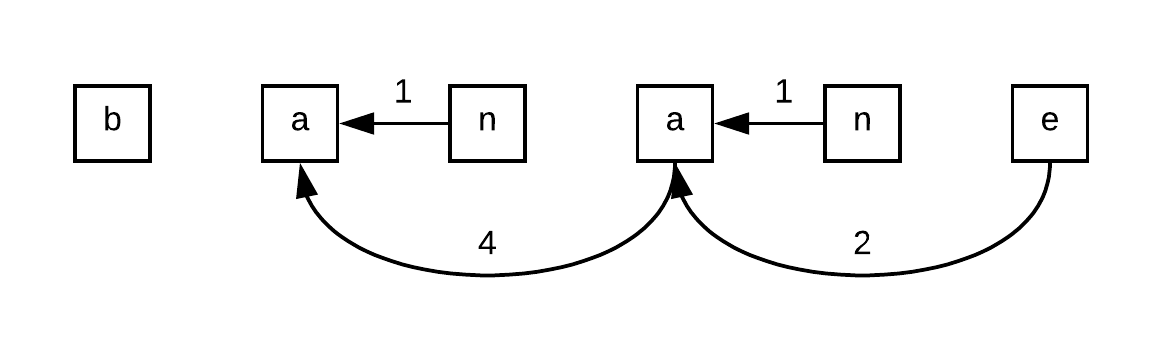
\includegraphics[width=10cm]{kapitel/saca_algorithmen/gsaca/images/Banane-prev-pointer}
	\end{minipage}
	\caption[Konstruktion des Suffix-Arrays für das Wort Banane: \prevpointer]{Konstruktion des Suffix-Arrays für das Wort Banane: \prevpointer. Die Zahlen geben die Nummer der Iteration an, in welcher der \prevpointer berechnet wurde.}
\label{fig_banane_prev_pointer}
\end{figure}
\newpage		% add new page to move the next section down
\newpage		% add new page to move the next section down
\newpage		% add new page to move the next section down

\subsection*{Phase 2:}
In der zweiten Phase wird das Suffix-Array mithilfe der zuvor erstellten Gruppen und Gruppenkontexte sowie der \prevpointer konstruiert. 
In diesem Beispiel werden hierfür 5 Iterationen durchlaufen.\\

Iteration 1:\\
Schritt 1: Die Abläufe der Phase 2 können an einer ähnlichen Tabelle visualisiert werden, wie dies bei Phase 1 der Fall war.
Die untere Hälfte der Tabelle enthält, genau wie die in Phase 1, das betrachtete Wort Banane und die Indices der Buchstaben. 
Die obere Hälfte besteht aus den Gruppen und Gruppenkontexten, wie sie aus Phase 1 übernommen wurden und aus der Liste \sa. 
Diese enthält den Index des ersten Buchstaben des Suffixes.
Wie zuvor beschrieben, werden in dieser Phase die Werte von \sa von links nach rechts durchlaufen, beginnend mit der ersten Gruppe, in diesem Beispiel also mit der Gruppe \textit{\$} an Index 7. 
Die Tabelle und die einzelnen Schritte dieser Iteration sind in Tabelle \ref{fig_banane_2_1} gezeigt. 
Die aktuell betrachtete Gruppe ist durch grünen Hintergrund gekennzeichnet. \\
Schritt 2: Es wird das Zeichen \textit{\$} an Position 7 im Wort Banane betrachtet. 
Auch die aktuell bearbeitete Position ist durch grüne Farbe hervorgehoben. \\
Schritt 3: Um das nächste Element von \sa zu bestimmen wird der direkte Vorgänger dieses Zeichens untersucht. 
Dabei bezieht sich diese Iteration also auf das Element 6, welches in der Zelle mit blauem Hintergrund zu sehen ist. \\
Schritt 4: Von diesem Element ausgehend werden die \prevpointer aus Phase 1 durchlaufen bis das letzte Element dieser Liste gefunden ist. 
Das Vorgängerelement von dem Zeichen \textit{e} an Index 6, also das Zeichen, auf das der \prevpointer von \textit{e} zeigt, ist das Zeichen \textit{a} an Index 4. 
Dieses wiederum hat einen \prevpointer auf das Zeichen \textit{a} an Index 2. 
Die betrachteten Indices, die in der Tabelle rot hinterlegt sind, werden in die Liste \sa übertragen. 
Somit enthält diese am Ende der ersten Iteration drei weitere Indices, welche durch gelben Hintergrund hervorgehoben sind. \\

Iteration 2:\\
Schritt 1: In diesem Durchlauf wird das zweite Element in \sa betrachtet, dies ist Index 2.\\
Schritt 2: Es wird dieser Index im Wort betrachtet.\\
Schritt 3: Der Vorgänger des Buchstaben \textit{a} an Index 2 ist das Zeichen \textit{b} an Index 1. 
Da \textit{b} kein vorheriges Element hat, der \prevpointer also auf kein Element zeigt, endet diese Iteration hier. 
Der Index von Zeichen \textit{b} wird in \sa eingetragen. Das Ergebnis lässt sich in Tabelle \ref{fig_banane_2_2} sehen.\\

Iteration 3: \\
Schritt 1: Als nächstes wird das dritte Element von \sa untersucht. 
Aus der Tabelle \ref{fig_banane_2_3} lässt sich erkennen, dass dies das Element an Index 4 ist.\\
Schritt 2: Das Zeichen an dem betrachteten Index ist \textit{a}.\\
Schritt 3: Der Vorgänger von \textit{a} an Index 4 ist \textit{n} an Index 3.\\
Schritt 4: Der \prevpointer von \textit{n} an Index 3 zeigt auf das \textit{a} an Index 2. 
Der Index 2 ist bereits in \sa enthalten, Index 3 aber noch nicht, daher wird dieser in die Liste aufgenommen.\\

Iteration 4: \\
Wie sich in der Tabellen \ref{fig_banane_2_4} sehen lässt, wird das Zeichen an Index 1 betrachtet. 
Dies ist das Zeichen \textit{b}, welches kein Element hat, auf das sein \prevpointer zeigt. 
Somit endet diese Iteration ohne Änderung der Tabelle.\\

Iteration 5: \\
Schritt 1: In dieser Iteration wird das Element an Index 6 untersucht.\\
Schritt 2: Das Zeichen an Index 6 im Wort ist \textit{e}.\\
Schritt 3: Es wird der Vorgänger von diesem Zeichen betrachtet. 
Die Tabelle zu dieser Iteration, Tabelle \ref{fig_banane_2_5}, zeigt, dass dies das Zeichen \textit{n} an Index 5 ist.\\
Schritt 4: Dieses Zeichen hat einen Zeiger auf das Vorgängerelement \textit{a} an Index 4. 
Wie in einer vorherigen Iteration hat dieses \textit{a} einen Zeiger auf das Zeichen \textit{a} an Index 2. 
Da die Zeichen an Index 4 und 2 bereits in der Liste \sa enthalten sind, wird in diesem Schritt nur der Index 5 zu dieser Liste hinzugefügt. 
Somit ist die Liste vollständig gefüllt.\\

In diesem einfachen und kurzen Beispiel weicht die Liste der Gruppen, welche das Ergebnis von Phase 2 ist, nicht von der Liste \sa ab.
Dies ist jedoch nicht immer der Fall, vor allem in längeren und komplexeren Beispielen unterscheiden sich diese teilweise. 
Diese Unterschiede werden bei der Berechnung des Suffix-Arrays für das Wort \textit{caabaccaabacaa} in Kapitel \ref{gsaca:chapter6} deutlich. 
Je mehr Gruppen mit mehr als einem Index existieren, umso häufiger kann die Reihenfolge der Indices innerhalb dieser Gruppe gewechselt werden. 
Im Beispiel zum Wort Banane gab es jedoch nur eine Gruppe mit mehr als einem Index. 
In dieser Gruppe mit dem Buchstaben n fand keine Veränderung durch diese Schritte statt.\\
\newpage

%%%%%%%%%%% Phase 2 %%%%%%%%%%%%%%%
\begin{table}[H]

\centering
\begin{adjustbox}{max width=\textwidth}
\begin{tabular}{ll}

% Phase 2 - Iteration 1 - Schritt 1
\begin{tabular}{lccccccc}
\multicolumn{8}{l}{Phase 2 - Iteration 1 - Schritt 1}                                                                                                                                             \\ \hline
\multicolumn{1}{l|}{Kontext} & \multicolumn{1}{c|}{\cellcolor[HTML]{\green}\$} & \multicolumn{1}{c|}{anane} & \multicolumn{1}{c|}{ane} & \multicolumn{1}{c|}{b} & \multicolumn{1}{c|}{e} & \multicolumn{2}{c}{n}    \\
\multicolumn{1}{l|}{Gruppe}  & \multicolumn{1}{c|}{\cellcolor[HTML]{\green}7}  & \multicolumn{1}{c|}{2}     & \multicolumn{1}{c|}{4}   & \multicolumn{1}{c|}{1} & \multicolumn{1}{c|}{6} & 3 & 5  \\ 
\multicolumn{1}{l|}{SA}      & \multicolumn{1}{c|}{\cellcolor[HTML]{\green}7}  & \multicolumn{1}{c|}{}      & \multicolumn{1}{c|}{}    & \multicolumn{1}{c|}{}  & \multicolumn{1}{c|}{}  &   &    \\ \hline
\multicolumn{1}{l|}{Index}   & 1                                               & 2                          & 3                        & 4                      & 5                      & 6 & 7  \\
\multicolumn{1}{l|}{Zeichen} & b                                               & a                          & n                        & a                      & n                      & e & \$
\end{tabular}

&

% Phase 2 - Iteration 1 - Schritt 2
\begin{tabular}{lccccccc}
\multicolumn{8}{l}{Phase 2 - Iteration 1 - Schritt 2}                                                                                                                                                                     \\ \hline
\multicolumn{1}{l|}{Kontext} & \multicolumn{1}{c|}{\cellcolor[HTML]{\green}\$} & \multicolumn{1}{c|}{anane} & \multicolumn{1}{c|}{ane} & \multicolumn{1}{c|}{b} & \multicolumn{1}{c|}{e} & \multicolumn{2}{c}{n}    \\
\multicolumn{1}{l|}{Gruppe}  & \multicolumn{1}{c|}{\cellcolor[HTML]{\green}7}  & \multicolumn{1}{c|}{2}     & \multicolumn{1}{c|}{4}   & \multicolumn{1}{c|}{1} & \multicolumn{1}{c|}{6} & 3 & 5                          \\ 
\multicolumn{1}{l|}{SA}      & \multicolumn{1}{c|}{\cellcolor[HTML]{\green}7}  & \multicolumn{1}{c|}{}      & \multicolumn{1}{c|}{}    & \multicolumn{1}{c|}{}  & \multicolumn{1}{c|}{}  &   &                            \\ \hline
\multicolumn{1}{l|}{Index}   & 1                                               & 2                          & 3                        & 4                      & 5                      & 6 & \cellcolor[HTML]{\green}7  \\
\multicolumn{1}{l|}{Zeichen} & b                                               & a                          & n                        & a                      & n                      & e & \cellcolor[HTML]{\green}\$
\end{tabular}

\\
&
\\

% Phase 2 - Iteration 1 - Schritt 3
\begin{tabular}{lccccccc}
\multicolumn{8}{l}{Phase 2 - Iteration 1 - Schritt 3}                                                                                                                                                                     \\ \hline
\multicolumn{1}{l|}{Kontext} & \multicolumn{1}{c|}{\cellcolor[HTML]{\green}\$} & \multicolumn{1}{c|}{anane} & \multicolumn{1}{c|}{ane} & \multicolumn{1}{c|}{b} & \multicolumn{1}{c|}{e} & \multicolumn{2}{c}{n} \\
\multicolumn{1}{l|}{Gruppe}  & \multicolumn{1}{c|}{\cellcolor[HTML]{\green}7}  & \multicolumn{1}{c|}{2}     & \multicolumn{1}{c|}{4}   & \multicolumn{1}{c|}{1} & \multicolumn{1}{c|}{6} & 3 & 5                          \\ 
\multicolumn{1}{l|}{SA}      & \multicolumn{1}{c|}{\cellcolor[HTML]{\green}7}  & \multicolumn{1}{c|}{}      & \multicolumn{1}{c|}{}    & \multicolumn{1}{c|}{}  & \multicolumn{1}{c|}{}  &   &                            \\ \hline
\multicolumn{1}{l|}{Index}   & 1                                               & 2                          & 3                        & 4                      & 5                      & \cellcolor[HTML]{\blue}6 & \cellcolor[HTML]{\green}7  \\
\multicolumn{1}{l|}{Zeichen} & b                                               & a                          & n                        & a                      & n                      & \cellcolor[HTML]{\blue}e & \cellcolor[HTML]{\green}\$
\end{tabular}

&

% Phase 2 - Iteration 1 - Schritt 4
\begin{tabular}{lccccccc}
\multicolumn{8}{l}{Phase 2 - Iteration 1 - Schritt 4}                                                                                                                                                                                                \\ \hline
\multicolumn{1}{l|}{Kontext} & \multicolumn{1}{c|}{\cellcolor[HTML]{\green}\$} & \multicolumn{1}{c|}{anane} & \multicolumn{1}{c|}{ane} & \multicolumn{1}{c|}{b}    & \multicolumn{1}{c|}{e} & \multicolumn{2}{c}{n}  \\
\multicolumn{1}{l|}{Gruppe}  & \multicolumn{1}{c|}{\cellcolor[HTML]{\green}7}  & \multicolumn{1}{c|}{2}     & \multicolumn{1}{c|}{4}   & \multicolumn{1}{c|}{1}    & \multicolumn{1}{c|}{6} & 3                         & 5                          \\ 
\multicolumn{1}{l|}{SA}      & \multicolumn{1}{c|}{\cellcolor[HTML]{\green}7}  & \multicolumn{1}{c|}{}      & \multicolumn{1}{c|}{}    & \multicolumn{1}{c|}{}     & \multicolumn{1}{c|}{}  &                           &                            \\ \hline
\multicolumn{1}{l|}{Index}   & 1                                               & \cellcolor[HTML]{\red}2  & 3                        & \cellcolor[HTML]{\red}4 & 5                      & \cellcolor[HTML]{\blue}6 & \cellcolor[HTML]{\green}7  \\
\multicolumn{1}{l|}{Zeichen} & b                                               & \cellcolor[HTML]{\red}a  & n                        & \cellcolor[HTML]{\red}a & n                      & \cellcolor[HTML]{\blue}e & \cellcolor[HTML]{\green}\$
\end{tabular}

\\
&
\\

% Phase 2 - Iteration 1 - Ergebnis
\begin{tabular}{lccccccc}
\multicolumn{8}{l}{Phase 2 - Iteration 1 - Ergebnis}                                                                                                                                                                                       \\ \hline
\multicolumn{1}{l|}{Kontext} & \multicolumn{1}{c|}{\$} & \multicolumn{1}{c|}{anane}                     & \multicolumn{1}{c|}{ane}                       & \multicolumn{1}{c|}{b} & \multicolumn{1}{c|}{e}                         & \multicolumn{2}{c}{n}   \\
\multicolumn{1}{l|}{Gruppe}  & \multicolumn{1}{c|}{7}  & \multicolumn{1}{c|}{2}                         & \multicolumn{1}{c|}{4}                         & \multicolumn{1}{c|}{1} & \multicolumn{1}{c|}{6}                         & 3 & 5  \\ 
\multicolumn{1}{l|}{SA}      & \multicolumn{1}{c|}{7}  & \multicolumn{1}{c|}{\cellcolor[HTML]{\yellow}2} & \multicolumn{1}{c|}{\cellcolor[HTML]{\yellow}4} & \multicolumn{1}{c|}{}  & \multicolumn{1}{c|}{\cellcolor[HTML]{\yellow}6} &   &    \\ \hline
\multicolumn{1}{l|}{Index}   & 1                       & 2                                              & 3                                              & 4                      & 5                                              & 6 & 7  \\
\multicolumn{1}{l|}{Zeichen} & b                       & a                                              & n                                              & a                      & n                                              & e & \$
\end{tabular}

\end{tabular}
\end{adjustbox}

\caption[Konstruktion des Suffix-Arrays für das Wort Banane: Phase 2, Iteration 1]{Konstruktion des Suffix-Arrays für das Wort Banane: Phase 2, Iteration 1}
\label{fig_banane_2_1} 
\end{table}

\begin{table}[H]

\centering
\begin{adjustbox}{max width=\textwidth}
\begin{tabular}{ll}

% Phase 2 - Iteration 2 - Schritt 1
\begin{tabular}{lccccccc}
\multicolumn{8}{l}{Phase 2 - Iteration 2 - Schritt 1}                                                                                                                                                             \\ \hline
\multicolumn{1}{l|}{Kontext} & \multicolumn{1}{c|}{\$} & \multicolumn{1}{c|}{\cellcolor[HTML]{\green}anane} & \multicolumn{1}{c|}{ane} & \multicolumn{1}{c|}{b} & \multicolumn{1}{c|}{e} & \multicolumn{2}{c}{n} \\
\multicolumn{1}{l|}{Gruppe}  & \multicolumn{1}{c|}{7}  & \multicolumn{1}{c|}{\cellcolor[HTML]{\green}2}     & \multicolumn{1}{c|}{4}   & \multicolumn{1}{c|}{1} & \multicolumn{1}{c|}{6} & 3         & 5          \\ 
\multicolumn{1}{l|}{SA}      & \multicolumn{1}{c|}{7}  & \multicolumn{1}{c|}{\cellcolor[HTML]{\green}2}     & \multicolumn{1}{c|}{4}   & \multicolumn{1}{c|}{}  & \multicolumn{1}{c|}{6} &           &            \\ \hline
\multicolumn{1}{l|}{Index}   & 1                       & 2                                                  & 3                        & 4                      & 5                      & 6         & 7          \\
\multicolumn{1}{l|}{Zeichen} & b                       & a                                                  & n                        & a                      & n                      & e         & \$        
\end{tabular}

&

% Phase 2 - Iteration 2 - Schritt 2
\begin{tabular}{lccccccc}
\multicolumn{8}{l}{Phase 2 - Iteration 2 - Schritt 2}                                                                                                                                                             \\ \hline
\multicolumn{1}{l|}{Kontext} & \multicolumn{1}{c|}{\$} & \multicolumn{1}{c|}{\cellcolor[HTML]{\green}anane} & \multicolumn{1}{c|}{ane} & \multicolumn{1}{c|}{b} & \multicolumn{1}{c|}{e} & \multicolumn{2}{c}{n} \\
\multicolumn{1}{l|}{Gruppe}  & \multicolumn{1}{c|}{7}  & \multicolumn{1}{c|}{\cellcolor[HTML]{\green}2}     & \multicolumn{1}{c|}{4}   & \multicolumn{1}{c|}{1} & \multicolumn{1}{c|}{6} & 3         & 5          \\
\multicolumn{1}{l|}{SA}      & \multicolumn{1}{c|}{7}  & \multicolumn{1}{c|}{\cellcolor[HTML]{\green}2}     & \multicolumn{1}{c|}{4}   & \multicolumn{1}{c|}{}  & \multicolumn{1}{c|}{6} &           &            \\ \hline
\multicolumn{1}{l|}{Index}   & 1                       & \cellcolor[HTML]{\green}2                          & 3                        & 4                      & 5                      & 6         & 7          \\
\multicolumn{1}{l|}{Zeichen} & b                       & \cellcolor[HTML]{\green}a                          & n                        & a                      & n                      & e         & \$        
\end{tabular}

\\
&
\\

% Phase 2 - Iteration 2 - Schritt 3
\begin{tabular}{lccccccc}
\multicolumn{8}{l}{Phase 2 - Iteration 2 - Schritt 3}                                                                                                                                                             \\ \hline
\multicolumn{1}{l|}{Kontext} & \multicolumn{1}{c|}{\$}   & \multicolumn{1}{c|}{\cellcolor[HTML]{\green}anane} & \multicolumn{1}{c|}{ane} & \multicolumn{1}{c|}{b} & \multicolumn{1}{c|}{e} & \multicolumn{2}{c}{n} \\
\multicolumn{1}{l|}{Gruppe}  & \multicolumn{1}{c|}{7}    & \multicolumn{1}{c|}{\cellcolor[HTML]{\green}2}     & \multicolumn{1}{c|}{4}   & \multicolumn{1}{c|}{1} & \multicolumn{1}{c|}{6} & 3         & 5         \\
\multicolumn{1}{l|}{SA}      & \multicolumn{1}{c|}{7}    & \multicolumn{1}{c|}{\cellcolor[HTML]{\green}2}     & \multicolumn{1}{c|}{4}   & \multicolumn{1}{c|}{}  & \multicolumn{1}{c|}{6} &           &            \\ \hline
\multicolumn{1}{l|}{Index}   & \cellcolor[HTML]{\blue}1 & \cellcolor[HTML]{\green}2                          & 3                        & 4                      & 5                      & 6         & 7          \\
\multicolumn{1}{l|}{Zeichen} & \cellcolor[HTML]{\blue}b & \cellcolor[HTML]{\green}a                          & n                        & a                      & n                      & e         & \$        
\end{tabular}

&

% Phase 2 - Iteration 2- Ergebnis
\begin{tabular}{lccccccc}
\multicolumn{8}{l}{Phase 2 - Iteration 2 - Ergebnis}                                                                                                                                                             \\ \hline
\multicolumn{1}{l|}{Kontext} & \multicolumn{1}{c|}{\$} & \multicolumn{1}{c|}{anane} & \multicolumn{1}{c|}{ane} & \multicolumn{1}{c|}{b}                         & \multicolumn{1}{c|}{e} & \multicolumn{2}{c}{n} \\
\multicolumn{1}{l|}{Gruppe}  & \multicolumn{1}{c|}{7}  & \multicolumn{1}{c|}{2}     & \multicolumn{1}{c|}{4}   & \multicolumn{1}{c|}{1}                         & \multicolumn{1}{c|}{6} & 3         & 5          \\ 
\multicolumn{1}{l|}{SA}      & \multicolumn{1}{c|}{7}    & \multicolumn{1}{c|}{2}     & \multicolumn{1}{c|}{4}   &  \multicolumn{1}{c|}{\cellcolor[HTML]{\yellow}1}   & \multicolumn{1}{c|}{6} &           &            \\ \hline
\multicolumn{1}{l|}{Index}   & 1                       & 2                          & 3                        & 4                                              & 5                      & 6         & 7          \\
\multicolumn{1}{l|}{Zeichen} & b                       & a                          & n                        & a                                              & n                      & e         & \$        
\end{tabular}

\end{tabular}
\end{adjustbox}

\caption[Konstruktion des Suffix Arrays f{\"u}r das Wort Banane: Phase 2, Iteration 2]{Konstruktion des Suffix Arrays f{\"u}r das Wort Banane: Phase 2, Iteration 2}
\label{fig_banane_2_2} 
\end{table}

\newpage 		% start new page to remove space between tables
\begin{table}[H]

\centering
\begin{adjustbox}{max width=\textwidth}
\begin{tabular}{ll}

% Phase 2 - Iteration 3 - Schritt 1
\begin{tabular}{lccccccc}
\multicolumn{8}{l}{Phase 2 - Iteration 3 - Schritt 1}                                                                                                                                                             \\ \hline
\multicolumn{1}{l|}{Kontext} & \multicolumn{1}{c|}{\$} & \multicolumn{1}{c|}{anane} & \multicolumn{1}{c|}{\cellcolor[HTML]{\green}ane} & \multicolumn{1}{c|}{b} & \multicolumn{1}{c|}{e} & \multicolumn{2}{c}{n} \\
\multicolumn{1}{l|}{Gruppe}  & \multicolumn{1}{c|}{7}  & \multicolumn{1}{c|}{2}     & \multicolumn{1}{c|}{\cellcolor[HTML]{\green}4}   & \multicolumn{1}{c|}{1} & \multicolumn{1}{c|}{6} & 3         & 5          \\ 
\multicolumn{1}{l|}{SA}      & \multicolumn{1}{c|}{7}  & \multicolumn{1}{c|}{2}     & \multicolumn{1}{c|}{\cellcolor[HTML]{\green}4}   & \multicolumn{1}{c|}{1} & \multicolumn{1}{c|}{6} &           &            \\ \hline
\multicolumn{1}{l|}{Index}   & 1                       & 2                          & 3                                                & 4                      & 5                      & 6         & 7          \\
\multicolumn{1}{l|}{Zeichen} & b                       & a                          & n                                                & a                      & n                      & e         & \$        
\end{tabular}

&

% Phase 2 - Iteration 3 - Schritt 2
\begin{tabular}{lccccccc}
\multicolumn{8}{l}{Phase 2 - Iteration 3 - Schritt 2}                                                                                                                                                                \\ \hline
\multicolumn{1}{l|}{Kontext} & \multicolumn{1}{c|}{\$} & \multicolumn{1}{c|}{anane} & \multicolumn{1}{c|}{\cellcolor[HTML]{\green}ane} & \multicolumn{1}{c|}{b}    & \multicolumn{1}{c|}{e} & \multicolumn{2}{c}{n} \\
\multicolumn{1}{l|}{Gruppe}  & \multicolumn{1}{c|}{7}  & \multicolumn{1}{c|}{2}     & \multicolumn{1}{c|}{\cellcolor[HTML]{\green}4}   & \multicolumn{1}{c|}{1}    & \multicolumn{1}{c|}{6} & 3         & 5          \\ 
\multicolumn{1}{l|}{SA}      & \multicolumn{1}{c|}{7}  & \multicolumn{1}{c|}{2}     & \multicolumn{1}{c|}{\cellcolor[HTML]{\green}4}   & \multicolumn{1}{c|}{1}    & \multicolumn{1}{c|}{6} &           &            \\ \hline
\multicolumn{1}{l|}{Index}   & 1                       & 2                          & 3                                                & \cellcolor[HTML]{\green}4 & 5                      & 6         & 7          \\
\multicolumn{1}{l|}{Zeichen} & b                       & a                          & n                                                & \cellcolor[HTML]{\green}a & n                      & e         & \$        
\end{tabular}

\\
&
\\

% Phase 2 - Iteration 3 - Schritt 3
\begin{tabular}{lccccccc}
\multicolumn{8}{l}{Phase 2 - Iteration 3 - Schritt 3}                                                                                                                                                                \\ \hline
\multicolumn{1}{l|}{Kontext} & \multicolumn{1}{c|}{\$} & \multicolumn{1}{c|}{anane} & \multicolumn{1}{c|}{\cellcolor[HTML]{\green}ane} & \multicolumn{1}{c|}{b}    & \multicolumn{1}{c|}{e} & \multicolumn{2}{c}{n} \\
\multicolumn{1}{l|}{Gruppe}  & \multicolumn{1}{c|}{7}  & \multicolumn{1}{c|}{2}     & \multicolumn{1}{c|}{\cellcolor[HTML]{\green}4}   & \multicolumn{1}{c|}{1}    & \multicolumn{1}{c|}{6} & 3         & 5          \\ 
\multicolumn{1}{l|}{SA}      & \multicolumn{1}{c|}{7}  & \multicolumn{1}{c|}{2}     & \multicolumn{1}{c|}{\cellcolor[HTML]{\green}4}   & \multicolumn{1}{c|}{1}    & \multicolumn{1}{c|}{6} &           &            \\ \hline
\multicolumn{1}{l|}{Index}   & 1                       & 2                          & \cellcolor[HTML]{\blue}3                        & \cellcolor[HTML]{\green}4 & 5                      & 6         & 7          \\
\multicolumn{1}{l|}{Zeichen} & b                       & a                          & \cellcolor[HTML]{\blue}n                        & \cellcolor[HTML]{\green}a & n                      & e         & \$        
\end{tabular}

&

% Phase 2 - Iteration 3 - Schritt 4
\begin{tabular}{lccccccc}
\multicolumn{8}{l}{Phase 2 - Iteration 3 - Schritt 4}                                                                                                                                                                \\ \hline
\multicolumn{1}{l|}{Kontext} & \multicolumn{1}{c|}{\$} & \multicolumn{1}{c|}{anane} & \multicolumn{1}{c|}{\cellcolor[HTML]{\green}ane} & \multicolumn{1}{c|}{b}    & \multicolumn{1}{c|}{e} & \multicolumn{2}{c}{n} \\
\multicolumn{1}{l|}{Gruppe}  & \multicolumn{1}{c|}{7}  & \multicolumn{1}{c|}{2}     & \multicolumn{1}{c|}{\cellcolor[HTML]{\green}4}   & \multicolumn{1}{c|}{1}    & \multicolumn{1}{c|}{6} & 3         & 5          \\ 
\multicolumn{1}{l|}{SA}      & \multicolumn{1}{c|}{7}  & \multicolumn{1}{c|}{2}     & \multicolumn{1}{c|}{\cellcolor[HTML]{\green}4}   & \multicolumn{1}{c|}{1}    & \multicolumn{1}{c|}{6} &           &            \\ \hline
\multicolumn{1}{l|}{Index}   & 1                       & \cellcolor[HTML]{\red}2  & \cellcolor[HTML]{\blue}3                        & \cellcolor[HTML]{\green}4 & 5                      & 6         & 7          \\
\multicolumn{1}{l|}{Zeichen} & b                       & \cellcolor[HTML]{\red}a  & \cellcolor[HTML]{\blue}n                        & \cellcolor[HTML]{\green}a & n                      & e         & \$        
\end{tabular}

\\
&
\\

% Phase 2 - Iteration 3 - Ergebnis
\begin{tabular}{lccccccc}
\multicolumn{8}{l}{Phase 2 - Iteration 3 - Ergebnis}                                                                                                                                             \\ \hline
\multicolumn{1}{l|}{Kontext} & \multicolumn{1}{c|}{\$} & \multicolumn{1}{c|}{anane} & \multicolumn{1}{c|}{ane} & \multicolumn{1}{c|}{b} & \multicolumn{1}{c|}{e} & \multicolumn{2}{c}{n}         \\
\multicolumn{1}{l|}{Gruppe}  & \multicolumn{1}{c|}{7}  & \multicolumn{1}{c|}{2}     & \multicolumn{1}{c|}{4}   & \multicolumn{1}{c|}{1} & \multicolumn{1}{c|}{6} & 3                         & 5  \\ 
\multicolumn{1}{l|}{SA}      & \multicolumn{1}{c|}{7}  & \multicolumn{1}{c|}{2}     & \multicolumn{1}{c|}{4}   & \multicolumn{1}{c|}{1} & \multicolumn{1}{c|}{6} & \cellcolor[HTML]{\yellow}3 &    \\ \hline
\multicolumn{1}{l|}{Index}   & 1                       & 2                          & 3                        & 4                      & 5                      & 6                         & 7  \\
\multicolumn{1}{l|}{Zeichen} & b                       & a                          & n                        & a                      & n                      & e                         & \$
\end{tabular}

\end{tabular}
\end{adjustbox}

\caption[Konstruktion des Suffix Arrays f{\"u}r das Wort Banane: Phase 2, Iteration 3]{Konstruktion des Suffix Arrays f{\"u}r das Wort Banane: Phase 2, Iteration 3}
\label{fig_banane_2_3} 
\end{table}

\begin{table}[H]

\centering
\begin{adjustbox}{max width=\textwidth}
\begin{tabular}{ll}

% Phase 2 - Iteration 4 - Schritt 1
\begin{tabular}{lccccccc}
\multicolumn{8}{l}{Phase 2 - Iteration 4 - Schritt 1}                                                                                                                                                             \\ \hline
\multicolumn{1}{l|}{Kontext} & \multicolumn{1}{c|}{\$} & \multicolumn{1}{c|}{anane} & \multicolumn{1}{c|}{ane} & \multicolumn{1}{c|}{\cellcolor[HTML]{\green}b} & \multicolumn{1}{c|}{e} & \multicolumn{2}{c}{n} \\
\multicolumn{1}{l|}{Gruppe}  & \multicolumn{1}{c|}{7}  & \multicolumn{1}{c|}{2}     & \multicolumn{1}{c|}{4}   & \multicolumn{1}{c|}{\cellcolor[HTML]{\green}1} & \multicolumn{1}{c|}{6} & 3         & 5          \\ 
\multicolumn{1}{l|}{SA}      & \multicolumn{1}{c|}{7}  & \multicolumn{1}{c|}{2}     & \multicolumn{1}{c|}{4}   & \multicolumn{1}{c|}{\cellcolor[HTML]{\green}1} & \multicolumn{1}{c|}{6} & 3         &            \\ \hline
\multicolumn{1}{l|}{Index}   & 1                       & 2                          & 3                        & 4                                              & 5                      & 6         & 7          \\
\multicolumn{1}{l|}{Zeichen} & b                       & a                          & n                        & a                                              & n                      & e         & \$        
\end{tabular}
&

% Phase 2 - Iteration 4 - Schritt 2
\begin{tabular}{lccccccc}
\multicolumn{8}{l}{Phase 2 - Iteration 4 - Schritt 2}                                                                                                                                                               \\ \hline
\multicolumn{1}{l|}{Kontext} & \multicolumn{1}{c|}{\$}   & \multicolumn{1}{c|}{anane} & \multicolumn{1}{c|}{ane} & \multicolumn{1}{c|}{\cellcolor[HTML]{\green}b} & \multicolumn{1}{c|}{e} & \multicolumn{2}{c}{n} \\
\multicolumn{1}{l|}{Gruppe}  & \multicolumn{1}{c|}{7}    & \multicolumn{1}{c|}{2}     & \multicolumn{1}{c|}{4}   & \multicolumn{1}{c|}{\cellcolor[HTML]{\green}1} & \multicolumn{1}{c|}{6} & 3         & 5          \\ 
\multicolumn{1}{l|}{SA}      & \multicolumn{1}{c|}{7}    & \multicolumn{1}{c|}{2}     & \multicolumn{1}{c|}{4}   & \multicolumn{1}{c|}{\cellcolor[HTML]{\green}1} & \multicolumn{1}{c|}{6} & 3         &            \\ \hline
\multicolumn{1}{l|}{Index}   & \cellcolor[HTML]{\green}1 & 2                          & 3                        & 4                                              & 5                      & 6         & 7          \\
\multicolumn{1}{l|}{Zeichen} & \cellcolor[HTML]{\green}b & a                          & n                        & a                                              & n                      & e         & \$        
\end{tabular}

\\
&
\\

% Phase 2 - Iteration 4 - Ergebnis
\begin{tabular}{lccccccc}
\multicolumn{8}{l}{Phase 2 - Iteration 4 - Ergebnis}                                                                                                                                     \\ \hline
\multicolumn{1}{l|}{Kontext} & \multicolumn{1}{c|}{\$} & \multicolumn{1}{c|}{anane} & \multicolumn{1}{c|}{ane} & \multicolumn{1}{c|}{b} & \multicolumn{1}{c|}{e} & \multicolumn{2}{c}{n} \\
\multicolumn{1}{l|}{Gruppe}  & \multicolumn{1}{c|}{7}  & \multicolumn{1}{c|}{2}     & \multicolumn{1}{c|}{4}   & \multicolumn{1}{c|}{1} & \multicolumn{1}{c|}{6} & 3         & 5          \\ 
\multicolumn{1}{l|}{SA}      & \multicolumn{1}{c|}{7}  & \multicolumn{1}{c|}{2}     & \multicolumn{1}{c|}{4}   & \multicolumn{1}{c|}{1} & \multicolumn{1}{c|}{6} & 3         &            \\ \hline
\multicolumn{1}{l|}{Index}   & 1                       & 2                          & 3                        & 4                      & 5                      & 6         & 7          \\
\multicolumn{1}{l|}{Zeichen} & b                       & a                          & n                        & a                      & n                      & e         & \$        
\end{tabular}

\end{tabular}
\end{adjustbox}

\caption[Konstruktion des Suffix Arrays f{\"u}r das Wort Banane: Phase 2, Iteration 4]{Konstruktion des Suffix Arrays f{\"u}r das Wort Banane: Phase 2, Iteration 4}
\label{fig_banane_2_4} 
\end{table}

\newpage 		% start new page to remove space between tables
\begin{table}[H]

\centering
\begin{adjustbox}{max width=\textwidth}
\begin{tabular}{ll}

% Phase 2 - Iteration 5 - Schritt 1
\begin{tabular}{lccccccc}
\multicolumn{8}{l}{Phase 2 - Iteration 5 - Schritt 1}                                                                                                                                                             \\ \hline
\multicolumn{1}{l|}{Kontext} & \multicolumn{1}{c|}{\$} & \multicolumn{1}{c|}{anane} & \multicolumn{1}{c|}{ane} & \multicolumn{1}{c|}{b} & \multicolumn{1}{c|}{\cellcolor[HTML]{\green}e} & \multicolumn{2}{c}{n} \\
\multicolumn{1}{l|}{Gruppe}  & \multicolumn{1}{c|}{7}  & \multicolumn{1}{c|}{2}     & \multicolumn{1}{c|}{4}   & \multicolumn{1}{c|}{1} & \multicolumn{1}{c|}{\cellcolor[HTML]{\green}6} & 3         & 5          \\
\multicolumn{1}{l|}{SA}      & \multicolumn{1}{c|}{7}  & \multicolumn{1}{c|}{2}     & \multicolumn{1}{c|}{4}   & \multicolumn{1}{c|}{1} & \multicolumn{1}{c|}{\cellcolor[HTML]{\green}6} & 3         &            \\ \hline
\multicolumn{1}{l|}{Index}   & 1                       & 2                          & 3                        & 4                      & 5                                              & 6         & 7          \\
\multicolumn{1}{l|}{Zeichen} & b                       & a                          & n                        & a                      & n                                              & e         & \$        
\end{tabular}

&

% Phase 2 - Iteration 5 - Schritt 2
\begin{tabular}{lccccccc}
\multicolumn{8}{l}{Phase 2 - Iteration 5 - Schritt 2}                                                                                                                                                                     \\ \hline
\multicolumn{1}{l|}{Kontext} & \multicolumn{1}{c|}{\$} & \multicolumn{1}{c|}{anane} & \multicolumn{1}{c|}{ane} & \multicolumn{1}{c|}{b} & \multicolumn{1}{c|}{\cellcolor[HTML]{\green}e} & \multicolumn{2}{c}{n}         \\
\multicolumn{1}{l|}{Gruppe}  & \multicolumn{1}{c|}{7}  & \multicolumn{1}{c|}{2}     & \multicolumn{1}{c|}{4}   & \multicolumn{1}{c|}{1} & \multicolumn{1}{c|}{\cellcolor[HTML]{\green}6} & 3                         & 5  \\ 
\multicolumn{1}{l|}{SA}      & \multicolumn{1}{c|}{7}  & \multicolumn{1}{c|}{2}     & \multicolumn{1}{c|}{4}   & \multicolumn{1}{c|}{1} & \multicolumn{1}{c|}{\cellcolor[HTML]{\green}6} & 3                         &    \\ \hline
\multicolumn{1}{l|}{Index}   & 1                       & 2                          & 3                        & 4                      & 5                                              & \cellcolor[HTML]{\green}6 & 7  \\
\multicolumn{1}{l|}{Zeichen} & b                       & a                          & n                        & a                      & n                                              & \cellcolor[HTML]{\green}e & \$
\end{tabular}

\\
&
\\

% Phase 2 - Iteration 5 - Schritt 3
\begin{tabular}{lccccccc}
\multicolumn{8}{l}{Phase 2 - Iteration 5 - Schritt 3}                                                                                                                                                                     \\ \hline
\multicolumn{1}{l|}{Kontext} & \multicolumn{1}{c|}{\$} & \multicolumn{1}{c|}{anane} & \multicolumn{1}{c|}{ane} & \multicolumn{1}{c|}{b} & \multicolumn{1}{c|}{\cellcolor[HTML]{\green}e} & \multicolumn{2}{c}{n}         \\
\multicolumn{1}{l|}{Gruppe}  & \multicolumn{1}{c|}{7}  & \multicolumn{1}{c|}{2}     & \multicolumn{1}{c|}{4}   & \multicolumn{1}{c|}{1} & \multicolumn{1}{c|}{\cellcolor[HTML]{\green}6} & 3                         & 5  \\ 
\multicolumn{1}{l|}{SA}      & \multicolumn{1}{c|}{7}  & \multicolumn{1}{c|}{2}     & \multicolumn{1}{c|}{4}   & \multicolumn{1}{c|}{1} & \multicolumn{1}{c|}{\cellcolor[HTML]{\green}6} & 3                         &    \\ \hline
\multicolumn{1}{l|}{Index}   & 1                       & 2                          & 3                        & 4                      & \cellcolor[HTML]{\blue}5                      & \cellcolor[HTML]{\green}6 & 7  \\
\multicolumn{1}{l|}{Zeichen} & b                       & a                          & n                        & a                      & \cellcolor[HTML]{\blue}n                      & \cellcolor[HTML]{\green}e & \$
\end{tabular}

&

% Phase 2 - Iteration 5 - Schritt 4
\begin{tabular}{lccccccc}
\multicolumn{8}{l}{Phase 2 - Iteration 5 - Schritt 1}                                                                                                                                                                        \\ \hline
\multicolumn{1}{l|}{Kontext} & \multicolumn{1}{c|}{\$} & \multicolumn{1}{c|}{anane} & \multicolumn{1}{c|}{ane} & \multicolumn{1}{c|}{b}    & \multicolumn{1}{c|}{\cellcolor[HTML]{\green}e} & \multicolumn{2}{c}{n}         \\
\multicolumn{1}{l|}{Gruppe}  & \multicolumn{1}{c|}{7}  & \multicolumn{1}{c|}{2}     & \multicolumn{1}{c|}{4}   & \multicolumn{1}{c|}{1}    & \multicolumn{1}{c|}{\cellcolor[HTML]{\green}6} & 3                         & 5  \\ 
\multicolumn{1}{l|}{SA}      & \multicolumn{1}{c|}{7}  & \multicolumn{1}{c|}{2}     & \multicolumn{1}{c|}{4}   & \multicolumn{1}{c|}{1}    & \multicolumn{1}{c|}{\cellcolor[HTML]{\green}6} & 3                         &    \\ \hline
\multicolumn{1}{l|}{Index}   & 1                       & \cellcolor[HTML]{\red}2  & 3                        & \cellcolor[HTML]{\red}4 & \cellcolor[HTML]{\blue}5                      & \cellcolor[HTML]{\green}6 & 7  \\
\multicolumn{1}{l|}{Zeichen} & b                       & \cellcolor[HTML]{\red}a  & n                        & \cellcolor[HTML]{\red}a & \cellcolor[HTML]{\blue}n                      & \cellcolor[HTML]{\green}e & \$
\end{tabular}

\\
&
\\

% Phase 2 - Iteration 5 - Ergebnis
\begin{tabular}{lccccccc}
\multicolumn{8}{l}{Phase 2 - Iteration 5 - Ergebnis}                                                                                                                                            \\ \hline
\multicolumn{1}{l|}{Kontext} & \multicolumn{1}{c|}{\$} & \multicolumn{1}{c|}{anane} & \multicolumn{1}{c|}{ane} & \multicolumn{1}{c|}{b} & \multicolumn{1}{c|}{e} & \multicolumn{2}{c}{n}        \\
\multicolumn{1}{l|}{Gruppe}  & \multicolumn{1}{c|}{7}  & \multicolumn{1}{c|}{2}     & \multicolumn{1}{c|}{4}   & \multicolumn{1}{c|}{1} & \multicolumn{1}{c|}{6} & 3 & 5                         \\ 
\multicolumn{1}{l|}{SA}      & \multicolumn{1}{c|}{7}  & \multicolumn{1}{c|}{2}     & \multicolumn{1}{c|}{4}   & \multicolumn{1}{c|}{1} & \multicolumn{1}{c|}{6} & 3 & \cellcolor[HTML]{\yellow}5 \\ \hline
\multicolumn{1}{l|}{Index}   & 1                       & 2                          & 3                        & 4                      & 5                      & 6 & 7                         \\
\multicolumn{1}{l|}{Zeichen} & b                       & a                          & n                        & a                      & n                      & e & \$                       
\end{tabular}

\end{tabular}
\end{adjustbox}

\caption[Konstruktion des Suffix-Arrays für das Wort Banane: Phase 2, Iteration 5]{Konstruktion des Suffix-Arrays für das Wort Banane: Phase 2, Iteration 5}
\label{fig_banane_2_5} 
\end{table}


%%%%%%%%%%% Ergebnis %%%%%%%%%%%%%%%
%\begin{table}[H]

\begin{center}
\begin{tabular}{l}

% Ergebnis der 2 Phasen
\begin{tabular}{lccccccc}
\multicolumn{8}{l}{Ergebnis der 2 Phasen}                                                                                                                                                                                                                                                                                                                        \\ \hline
\rowcolor[HTML]{\red} 
\multicolumn{1}{l|}{\cellcolor[HTML]{\red}Kontext} & \multicolumn{1}{c|}{\cellcolor[HTML]{\red}\$} & \multicolumn{1}{c|}{\cellcolor[HTML]{\red}anane} & \multicolumn{1}{c|}{\cellcolor[HTML]{\red}ane} & \multicolumn{1}{c|}{\cellcolor[HTML]{\red}b} & \multicolumn{1}{c|}{\cellcolor[HTML]{\red}e} & \multicolumn{2}{c}{\cellcolor[HTML]{\red}n} \\
\rowcolor[HTML]{\white} 
\multicolumn{1}{l|}{\cellcolor[HTML]{\white}Gruppe}  & \multicolumn{1}{c|}{\cellcolor[HTML]{\white}7}  & \multicolumn{1}{c|}{\cellcolor[HTML]{\white}2}     & \multicolumn{1}{c|}{\cellcolor[HTML]{\white}4}   & \multicolumn{1}{c|}{\cellcolor[HTML]{\white}1} & \multicolumn{1}{c|}{\cellcolor[HTML]{\white}6} & 3                     & 5                     \\
\rowcolor[HTML]{\gray} 
\multicolumn{1}{l|}{\cellcolor[HTML]{\gray}SA}      & \multicolumn{1}{c|}{\cellcolor[HTML]{\gray}7}  & \multicolumn{1}{c|}{\cellcolor[HTML]{\gray}2}     & \multicolumn{1}{c|}{\cellcolor[HTML]{\gray}4}   & \multicolumn{1}{c|}{\cellcolor[HTML]{\gray}1} & \multicolumn{1}{c|}{\cellcolor[HTML]{\gray}6} & 3                     & 5                     \\ \cline{2-8} 
\rowcolor[HTML]{\yellow} 
\multicolumn{1}{l|}{\cellcolor[HTML]{\yellow}Index}   & 1                                               & 2                                                  & 3                                                & 4                                              & 5                                              & 6                     & 7                     \\
\rowcolor[HTML]{\green} 
\multicolumn{1}{l|}{\cellcolor[HTML]{\green}Zeichen} & b                                               & a                                                  & n                                                & a                                              & n                                              & e                     & \$                   
\end{tabular}

\\
\\

% Endergebnis - Schritt 1
\begin{tabular}{cccccc}
\multicolumn{6}{l}{Endergebnis - Schritt 1}                                                                                                                 \\
\cellcolor[HTML]{\green}Zeichen & \cellcolor[HTML]{\yellow}Index & \cellcolor[HTML]{\gray}SA & $ \widehat{SA} $ & S\textsubscript{SA} & \cellcolor[HTML]{\red}S{[}SA..$ \widehat{SA} $ {]} \\
\cellcolor[HTML]{\green}b       & \cellcolor[HTML]{\yellow}1     & \cellcolor[HTML]{\gray}7  &    &     & \cellcolor[HTML]{\red}\$            \\
\cellcolor[HTML]{\green}a       & \cellcolor[HTML]{\yellow}2     & \cellcolor[HTML]{\gray}2  &    &     & \cellcolor[HTML]{\red}anane         \\
\cellcolor[HTML]{\green}n       & \cellcolor[HTML]{\yellow}3     & \cellcolor[HTML]{\gray}4  &    &     & \cellcolor[HTML]{\red}ane           \\
\cellcolor[HTML]{\green}a       & \cellcolor[HTML]{\yellow}4     & \cellcolor[HTML]{\gray}1  &    &     & \cellcolor[HTML]{\red}b             \\
\cellcolor[HTML]{\green}n       & \cellcolor[HTML]{\yellow}5     & \cellcolor[HTML]{\gray}6  &    &     & \cellcolor[HTML]{\red}e             \\
\cellcolor[HTML]{\green}e       & \cellcolor[HTML]{\yellow}6     & \cellcolor[HTML]{\gray}3  &    &     & \cellcolor[HTML]{\red}n             \\
\cellcolor[HTML]{\green}\$      & \cellcolor[HTML]{\yellow}7     & \cellcolor[HTML]{\gray}5  &    &     & \cellcolor[HTML]{\red}n            
\end{tabular}

\\
\\

% Endergebnis - Schritt 2
\begin{tabular}{cccccc}
\multicolumn{6}{l}{Endergebnis - Schritt 2}                                                                                                                 \\
Zeichen & Index & SA & \cellcolor[HTML]{\blue} $ \widehat{SA} $ & S\textsubscript{SA} & S{[}SA..$ \widehat{SA} $ {]} \\
b       & 1     & 7  & \cellcolor[HTML]{\blue}8  &     & \$            \\
a       & 2     & 2  & \cellcolor[HTML]{\blue}7  &     & anane         \\
n       & 3     & 4  & \cellcolor[HTML]{\blue}7  &     & ane           \\
a       & 4     & 1  & \cellcolor[HTML]{\blue}2  &     & b             \\
n       & 5     & 6  & \cellcolor[HTML]{\blue}7  &     & e             \\
e       & 6     & 3  & \cellcolor[HTML]{\blue}4  &     & n             \\
\$      & 7     & 5  & \cellcolor[HTML]{\blue}6  &     & n              
\end{tabular}

\\
\\

% Endergebnis - Schritt 3
\begin{tabular}{cccccc}
\multicolumn{6}{l}{Endergebnis - Schritt 3}                                                                                                                 \\
Zeichen & Index & SA & $ \widehat{SA} $ & S\textsubscript{SA} & S{[}SA..$ \widehat{SA} $ {]} \\ \cline{5-5}
b       & 1     & 7  & \multicolumn{1}{c|}{8} & \multicolumn{1}{c|}{\$}       & \$            \\
a       & 2     & 2  & \multicolumn{1}{c|}{7} & \multicolumn{1}{c|}{anane\$}  & anane         \\
n       & 3     & 4  & \multicolumn{1}{c|}{7} & \multicolumn{1}{c|}{ane\$}    & ane           \\
a       & 4     & 1  & \multicolumn{1}{c|}{2} & \multicolumn{1}{c|}{banane\$} & b             \\
n       & 5     & 6  & \multicolumn{1}{c|}{7} & \multicolumn{1}{c|}{e\$}      & e             \\
e       & 6     & 3  & \multicolumn{1}{c|}{4} & \multicolumn{1}{c|}{nane\$}   & n             \\
\$      & 7     & 5  & \multicolumn{1}{c|}{6} & \multicolumn{1}{c|}{ne\$}     & n             \\ \cline{5-5}
\end{tabular}

\end{tabular}
\end{center}

\caption[Konstruktion des Suffix Arrays für das Wort Banane: Zusammenführen der Ergebnisse]{Konstruktion des Suffix Arrays für das Wort Banane: Zusammenführen der Ergebnisse}
\label{fig_banane_2_end}
\end{table}
